\documentclass[10pt,a4paper,final]{article}
\usepackage[utf8]{inputenc}
\usepackage[portuguese]{babel}
\usepackage[T1]{fontenc}
\usepackage[margin=1in]{geometry}
\usepackage{amsmath}
\usepackage{amsfonts}
\usepackage[table]{xcolor}
\usepackage{graphicx}
\usepackage{multirow}
\usepackage{setspace}
\usepackage{amssymb}
\usepackage{lscape}
\usepackage{plano}
%\usepackage[alf]{abntex2cite}
\usepackage{natbib}
\usepackage{hyperref}
\usepackage{csquotes}

\programa{Engenharia Elétrica}
\area{Engenharia de Computação}
\aluno{Jefferson Carlos de Mendonça}
\orientador{Edson Satoshi Gomi}
\curso{Mestrado}
\dataIngresso{14/09/2016}
\titulo{Categorização das Perguntas do \textit{Site Stack Overflow}}
\resumo{
Transformações no cenário tecnológico provocam mudanças constantes que exigem atualização contínua. Para manter-se atualizado, profissionais da área de computação recorrem à diversas fontes de informação, dentre elas destaca-se o site \textit{Stack Overflow}\footnote{\url{http://stackoverflow.com/tour}}, maior comunidade de perguntas e respostas, onde os usuários podem aprender, trocar experiências e compartilhar conhecimento.
O objeto de pesquisa deste trabalho é propor um algoritmo que consiga categorizar as perguntas deste \textit{website}. Uma vez que os questionamentos estejam devidamente indexados e organizados em tópicos, será possível detectar as dúvidas mais frequêntes reportadas pelos usuários, além de permitir, que os motores de busca encontrem um assunto de interesse com maior facilidade.}

\palavrachave{recuperação de informação}
\palavrachave{mineração de textos}
\palavrachave{classificação de textos}
\palavrachave{categorização automática de textos}
\palavrachave{extração de palavras chave}
\palavrachave{indexação de documentos}
\palavrachave{stack overflow}


\begin{document}

    \folhaDeRosto

    \plano
    
    \section{Introdução}
    
A evolução na área computacional se desenvolve em ritmo acelerado, novos algoritmos, técnicas para programação distribuída, testes automatizados, bancos de dados etc. são assuntos que mudam com frequência, sem contar as \emph{linguagens de programação} que aprimoram suas API's constantemente, construindo e desconstruindo métodos e muitas vezes incorporam novos paradigmas. Para acompanhar as constantes mudanças, profissionais da área de computação necessitam qualificação, que pode ser obtida através de cursos presenciais, a distância, livros, revistas, artigos e claro \textit{websites}. \cite{Manning2009} afirma que a \textit{web} tornou-se a principal fonte por busca de informação e o relatório elaborado por \cite{Fallows} conclui que \enquote{ 92\% dos internautas dizem que a internet é um bom lugar para obter informações diariamente }.
Dentre estas fontes, merece destaque o fórum \textit{Stack Overflow} (SO), maior comunidade \textit{online} de perguntas e respostas onde os usuários podem aprender, trocar experiências e compartilhar conhecimento.
    
    \subsection{Contextualização do Problema}
O número de questões em sites de perguntas e respostas cresce diariamente, faz-se necessário categorizar os assuntos discutidos em tópicos, para uma busca mais eficiente e rápida. \cite{Manning2009} compara este problema ao da procura de um livro em uma biblioteca, com certeza nossa busca será mais rápida e assertiva se os livros estiverem separados em prateleiras por assunto ou tópico. \cite{Yasotha2016} adiciona que, a categorização manual de textos, pode ser feita somente por especialistas e requer muito tempo. Como consequência é de grande importância a categorização e classificação de documentos de forma automática ajudando os usuários a encontrarem informações relevantes para as suas necessidades.

    \subsection{Objetivos}
Propor um algoritmo capaz de categorizar de forma automática as perguntas de um site como o SO.

    \subsection{Justificativas}

O método proposto por \cite{Arash2016} categoriza os dados do SO. Em seu projeto os autores classificaram os assuntos utilizando as tags da própria pergunta, e então eles utilizaram o site Wikipédia para validar o tópico encontrado, assim foi possível identificar qual categoria uma pergunta pertence. No SO o próprio usuário, elege qual é a tag da referida pergunta publicada, limitando a expansão da solução existente para categorizar \textit{posts} em fórums que não possuem este recurso, exemplos: Code Ranch e Quora.
\newline
\newline
A proposta deste projeto de pequisa, é desenvolver um algoritmo em que a categorização e classificação dos assuntos discutidos no SO faça uso apenas do texto disponível nas perguntas e respostas, sem que haja a necessidade de recorrer ao uso de tags, desta forma será possível replicar a solução em outros \textit{sites}.

   \subsection{Organização do texto}

Para melhor definir qual o posicionamento do presente projeto, no capítulo seguinte será detalhado em maior profundidade os projetos que abordaram a categorização de documentos, inclusive àqueles que também fizeram uso do site \textit{Stack Overflow} como base de dados. Então a proposta será detalhada quantos aos procedimentos para a indexação das perguntas e respostas, desde a seleção do conteúdo original, armazenamento em banco de dados e extração, por fim serão exibidos os resultados esperados. Segundo \cite{Kaleta2014} o termo indexação pode ser entendido como um dicionário de palavras-chave que representam o conteúdo de um texto.	

 \section{Revisão da Literatura}
   


 \section{Detalhamento da Proposta}

Aqui deve-se descrever a metodologia.


%%\begin{figure}[!htb] 
%%\centering
%%    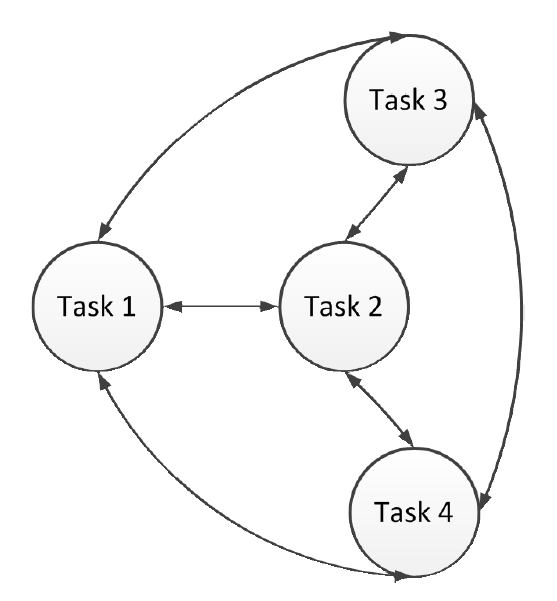
\includegraphics[height=5cm]{Figures/PTL}\label{fig:PTL}   
%% \caption{Fluxo de conhecimento na T L com transferência paralela (PTL).}
%%\end{figure}

  
    \section{Plano de Trabalho}



    \subsection{Resultados Desejados e Validação}
    
A análise será feita sobre os mesmo dados da pesquisa realizada por \cite{Arash2016}, os resultados obtidos anteriormente serão a base para a medição da acurácia da nova proposta e então será possível aplicar o modelo desenvolvido sem a utilização de tags pré-definidas, possibilitando a construção de catálogos para outros sites de perguntas e respostas.
 
    \subsection{Atividades e Cronograma}
    
Atividades e Cronograma.



% ----------------------------------------------------------
% Referências bibliográficas
% ----------------------------------------------------------
\nocite{Joorabchi2015}
\nocite{Manning2009}
\nocite{Mihalcea2007}
\nocite{Mihalcea2001}
\nocite{Mihalcea2004}
\nocite{Miotto2013}
\nocite{Posch2014}
\nocite{Roul2015}
\nocite{Udell2005}
\nocite{Kaleta2014}
\bibliographystyle{apalike}
\bibliography{Refs}{}  


    

\end{document}
    